IMAP4 ist die Version 4 des \QuoteM{INTERNET MESSAGE ACCESS PROTOCOL} spezifiziert in RFC 3501 \RefIt{rfc3501}. Es ist ähnlich wie POP3 ein textbasiertes Client-Server Protokoll, das das Auflisten, Löschen und Manipulieren von E-Mails an einem E-Mail Server erlaubt, weit über die Möglichkeiten von POP3 hinaus \QuoteIndirect{rfc1939}{S. 2}.

Ein E-Mail Server kann sowohl POP3 als auch IMAP4 gleichzeitig anbieten. Im Gegensatz zu POP3 erlaubt IMAP4 allerdings nicht nur E-Mails herunterzuladen, zu löschen oder aufzulisten, sondern direkt auf der Mailbox des E-Mail Servers zu operieren, was Funktionalitäten wie neue Ordner anzulegen erlaubt \QuoteIndirect{rfc3501}{S. 34 f} oder das serverseitige Durchsuchen von Nachrichten \QuoteIndirect{rfc3501}{S. 49 ff}.

Informationen werden nach Bedarf direkt vom IMAP4 Server abgerufen und nicht einzeln heruntergeladen. Deshalb ist auch im Gegensatz zu POP3 eine lokale Speicherung von Daten nicht notwendig, welche auch dazu führen kann, dass die lokale Mailbox von der entfernten Mailbox divergiert. E-Mail Programme bieten jedoch unabhängig von POP3/IMAP4 die Möglichkeit der lokalen Speicherung an, was allerdings Protokoll-agnostisch ist. Bei IMAP4 ist anzumerken, dass bei fehlender Internetverbindung und keiner expliziten lokalen Speicherung auf Programmebene der Zugriff auf E-Mails auch nicht mehr möglich ist.

IMAP4 benötigt ein zuverlässiges Netzwerkprotokoll wie beispielsweise TCP und wird über den Port 143 abgewickelt \QuoteIndirect{rfc3501}{S. 6}. Ist die Verbindung über IMAPS TLS/SSL-verschlüsselt wird häufig Port 993 benutzt, obwohl in RFC 2595 \RefIt{rfc2595} STARTTLS über den Standardport 143 beworben wird.

Ebenso wie POP3 ist auch IMAP4 ein zustandsbehaftetes Protokoll. Allerdings ist IMAP4 weitaus komplexer und kann sich in 4 verschiedenen Zuständen befinden. Wenn die Verbindung vom Client zum Server initial erstellt wurde, befindet sich die Kommunikation im \QuoteDirect{Not Authenticated State}{rfc3501}{S. 13}. Es wird vom Client nun erwartet, sich zu authentifizieren. Findet eine erfolgreiche Authentifizierung statt, so wird der \QuoteDirect{Authenticated State}{rfc3501}{S. 13} erreicht. Nachfolgend muss der Client eine Mailbox auswählen, bevor er weitere Kommandos zur Manipulation oder Einsicht von E-Mails abgeben kann. Ebenso wird dieser Zustand erreicht, wenn es einen Fehler beim Auswählen einer Mailbox gab oder nach einem erfolgreichen \verb#CLOSE# Kommando \QuoteIndirect{rfc3501}{S. 13}. Wurde eine Mailbox erfolgreich ausgewählt, so erreicht die Verbindung den \QuoteDirect{Selected State}{rfc3501}{S. 13}. In diesem Zustand kann auf der Mailbox operiert werden wie z.B. Ordner anlegen, E-Mails abrufen etc. Der letzte Zustand ist der \QuoteDirect{Logout State}{rfc3501}{S. 14} und kann aus allen vorherigen Zuständen erreicht werden. Hier wird die Verbindung terminiert.

Eine vereinfachte Darstellung der Kommunikation in einem SDL Diagramm ist in \autoref{fig:imap4} zu sehen. Diese Abbildung zeigt bereits die Komplexität des Protokolls, ist aber nicht vollständig. Deshalb kann an dieser Stelle aufgrund der Vielzahl möglicher Kommandos keine vollständige Betrachtung vorgenommen werden. Stattdessen wird nachfolgend eine einfache IMAP4 Sitzung betrachtet:

\begin{minipage}{\linewidth}
\begin{mail}{IMAP4-Sitzung}{IMAP4-Sitzung}
C: <öffnet Verbindung>
S: * OK IMAP4rev1 Service Ready
C: a001 login mrc secret
S: a001 OK LOGIN completed
C: a002 select inbox
S: * 322 EXISTS
S: * FLAGS (\Answered \Flagged \Deleted \Seen \Draft)
S: * 12 RECENT
S: * OK [UNSEEN 88] Message 88 is the first unseen message
S: a002 OK [READ-WRITE] SELECT completed
C: a003 fetch 8 body[header]
S: * 8 FETCH (BODY[HEADER] {342} 
S: From: Hans Bauer <hans@bauer.de>
S: To: Mina Meier <mina@meier.de>,
S:     Kaiser Wilhelm <wilhelm@keiser.de>
S: Date: Tue, 8 Mar 2016 06:46:18 -0800
S: Subject: Beispiel-Mail
S: Message-ID: <18283.122131@bauer.de>
S: X-Mein-Header: True
S:
S: )
S: a003 OK FETCH completed
C: a004 store 8 +flags \deleted
S: * 8 FETCH (FLAGS (\Seen \Deleted))
S: a004 OK +FLAGS completed
C: a005 logout
S: * BYE IMAP4rev1 server terminating connection
S: a005 OK LOGOUT completed     
\end{mail}
\end{minipage}

Wie hier zu sehen ist, sind die Transaktionen durchnummeriert und haben für Client und Server denselben Bezeichner. Der IMAP4 Zustand ist implizit und muss aus dem Kontext erschlossen werden.

% TODO: figure gets misplaced
% TODO: nicht alle server Nachrichten dargestellt
\begin{figure}[htb]
	%\Centerfloat
	\centering
	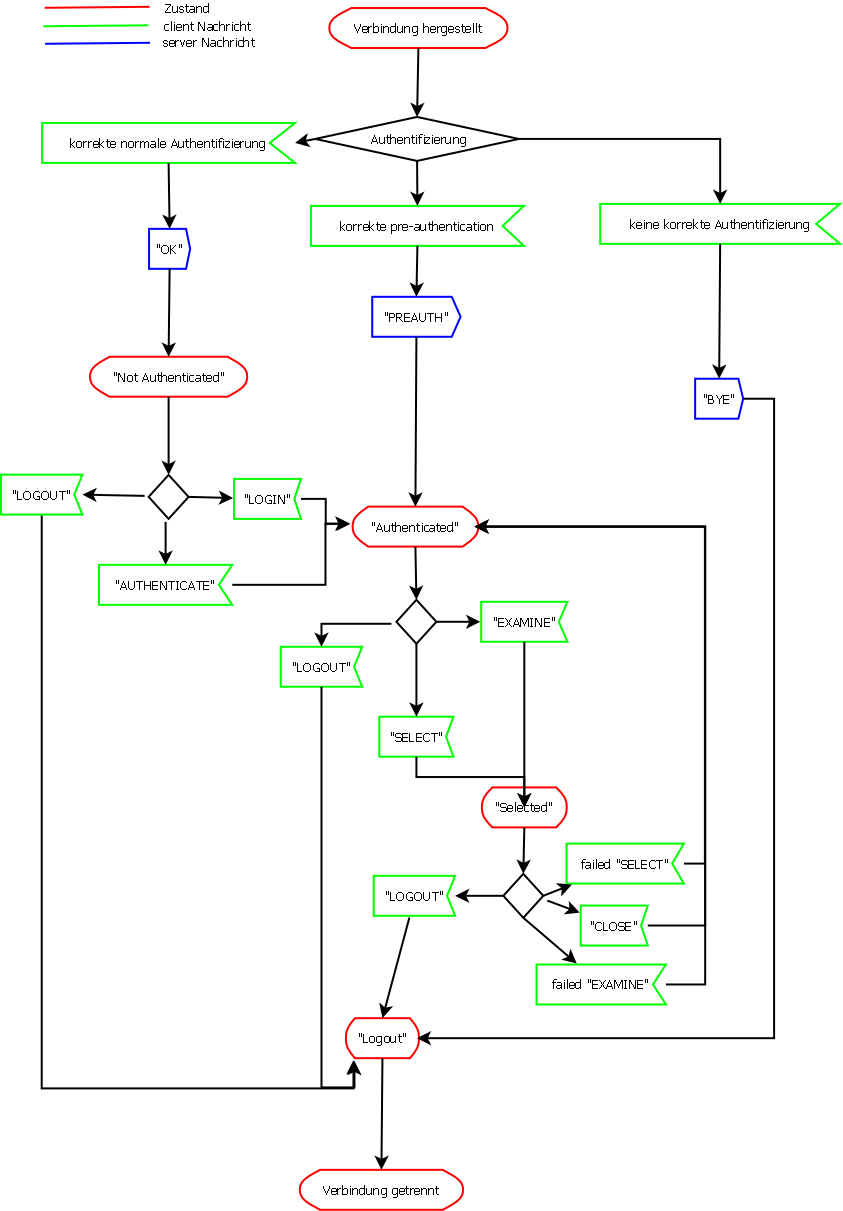
\includegraphics[scale=0.4]{Content/Intro/Protokolle/IMAP4.png}
	\caption{IMAP4 SDL Diagramm}
	\label{fig:imap4}
\end{figure}

\vfill
\clearpage
